% ============================================================================
%  cEatsv2-intel - Documentacion del proyecto final
%  Programacion II (V2214) - Programacion Orientada a Objetos
%  Compilar con:  latexmk -pdf proyecto.tex     (o pdflatex dos veces)
%  Requiere las imagenes exportadas en ../uml/png/*.png
% ============================================================================
\documentclass[11pt,letterpaper]{article}

\usepackage[utf8]{inputenc}
\usepackage[T1]{fontenc}
\usepackage[spanish,es-noquoting]{babel}
\usepackage[margin=2.5cm]{geometry}
\usepackage{graphicx}
\usepackage{float}
\usepackage{booktabs}
\usepackage{longtable}
\usepackage{listings}
\usepackage{xcolor}
\usepackage{amsmath,amssymb}
\usepackage{hyperref}
\usepackage{fancyhdr}

\hypersetup{colorlinks=true, linkcolor=black, urlcolor=blue, citecolor=black}

\definecolor{codebg}{RGB}{248,248,248}
\definecolor{codekw}{RGB}{0,90,160}
\definecolor{codecm}{RGB}{110,110,110}
\definecolor{codestr}{RGB}{160,60,20}

\lstdefinestyle{py}{
  language=Python,
  backgroundcolor=\color{codebg},
  basicstyle=\ttfamily\footnotesize,
  keywordstyle=\color{codekw}\bfseries,
  commentstyle=\color{codecm}\itshape,
  stringstyle=\color{codestr},
  numbers=left, numberstyle=\tiny\color{codecm}, numbersep=8pt,
  frame=single,
  breaklines=true, showstringspaces=false,
  inputencoding=utf8, extendedchars=true,
  literate=%
    {á}{{\'a}}1 {é}{{\'e}}1 {í}{{\'i}}1 {ó}{{\'o}}1 {ú}{{\'u}}1
    {ñ}{{\~n}}1 {Á}{{\'A}}1 {É}{{\'E}}1 {Í}{{\'I}}1 {Ó}{{\'O}}1
    {Ú}{{\'U}}1 {Ñ}{{\~N}}1
}
\lstset{style=py}

\pagestyle{fancy}
\fancyhf{}
\lhead{\small cEatsv2-intel}
\rhead{\small Programación II --- POO}
\cfoot{\thepage}

\begin{document}

% ------------------------------------------------------------------ PORTADA
\begin{titlepage}
\centering
\vspace*{2cm}
{\Huge\bfseries cEatsv2-intel\par}
\vspace{0.6cm}
{\Large Microservicio de recomendaciones y analítica para cEats\par}
\vspace{1.5cm}
{\large Proyecto final de Programación II (V2214)\par}
{\large Programación Orientada a Objetos\par}
\vspace{1.5cm}
\begin{tabular}{rl}
\textbf{Alumno:} & Paulo Cruz \\
\textbf{Profesora:} & \rule{5cm}{0.4pt} \\
\textbf{Lenguaje:} & Python 3.12 \\
\textbf{Repositorio:} & \texttt{github.com/CesarCrz/cEatsv2-intel} \\
\textbf{Despliegue:} & VPS propio (Docker / EasyPanel) \\
\textbf{Fecha:} & \today \\
\end{tabular}
\vfill
\end{titlepage}

\tableofcontents
\newpage

% ------------------------------------------------------------------ RESUMEN
\section{De qué trata}

cEats es una plataforma de pedidos que opera en producción, con restaurantes
reales y clientes reales. Una de sus funciones sugiere productos durante el
checkout: el cliente arma su carrito y antes de pagar le aparecen dos o tres
cosas que podría agregar.

El problema está en cómo las escoge. Hoy cuenta cuántas veces dos productos
salieron juntos en el mismo pedido, y con eso arma la lista. El resultado es que
el refresco gana siempre, porque el refresco sale con todo. No porque el cliente
haya pedido tacos, sino porque casi todos piden refresco.

Lo que quiero medir es distinto: cuánto sube la probabilidad de que pidan B
\emph{porque} pidieron A. Esa medida se llama \emph{lift} y es la base del
análisis de canasta de mercado.

\texttt{cEatsv2-intel} es el servicio que hace ese cálculo. Está escrito en
Python, con arquitectura por capas y programación orientada a objetos, y vive
aparte del backend. Ya que carga el historial de ventas para calcular el lift,
aprovecha para resolver dos cosas más: cuántos pedidos se esperan por hora en
cada sucursal, y qué productos dan dinero contra cuáles sólo ocupan espacio en
el menú.

La parte analítica (soporte, confianza, lift, series de tiempo y detección de
anomalías por puntaje $z$) es lo que cubre el requisito de la Unidad 4 de
resolver un problema aplicado de ciencia de datos.

\subsection{Por qué un servicio aparte}
La lógica analítica estaba mezclada con la capa HTTP del backend, y así no se
puede probar sin levantar el servidor completo. Separándola queda un dominio que
corre con \texttt{pytest} en dos segundos y sin red.

El costo de separarla es que ahora hay una llamada de red que puede fallar. Eso
se resuelve degradando: si el servicio no responde a tiempo, el backend usa el
resolutor viejo y el checkout ni se entera.

\newpage
% ------------------------------------------------------------------ UNIDAD 1
\section{Unidad 1 --- Fundamentos de POO}

\subsection{Resultado de aprendizaje}
Distinguir los conceptos básicos de la programación orientada a objetos para
fundamentar el diseño de clases y estructuras.

\subsection{Diseño de clases del dominio}
El dominio modela el negocio real de cEats: productos, pedidos, líneas de
pedido, canastas, sucursales e historial de ventas.

\begin{figure}[H]
\centering
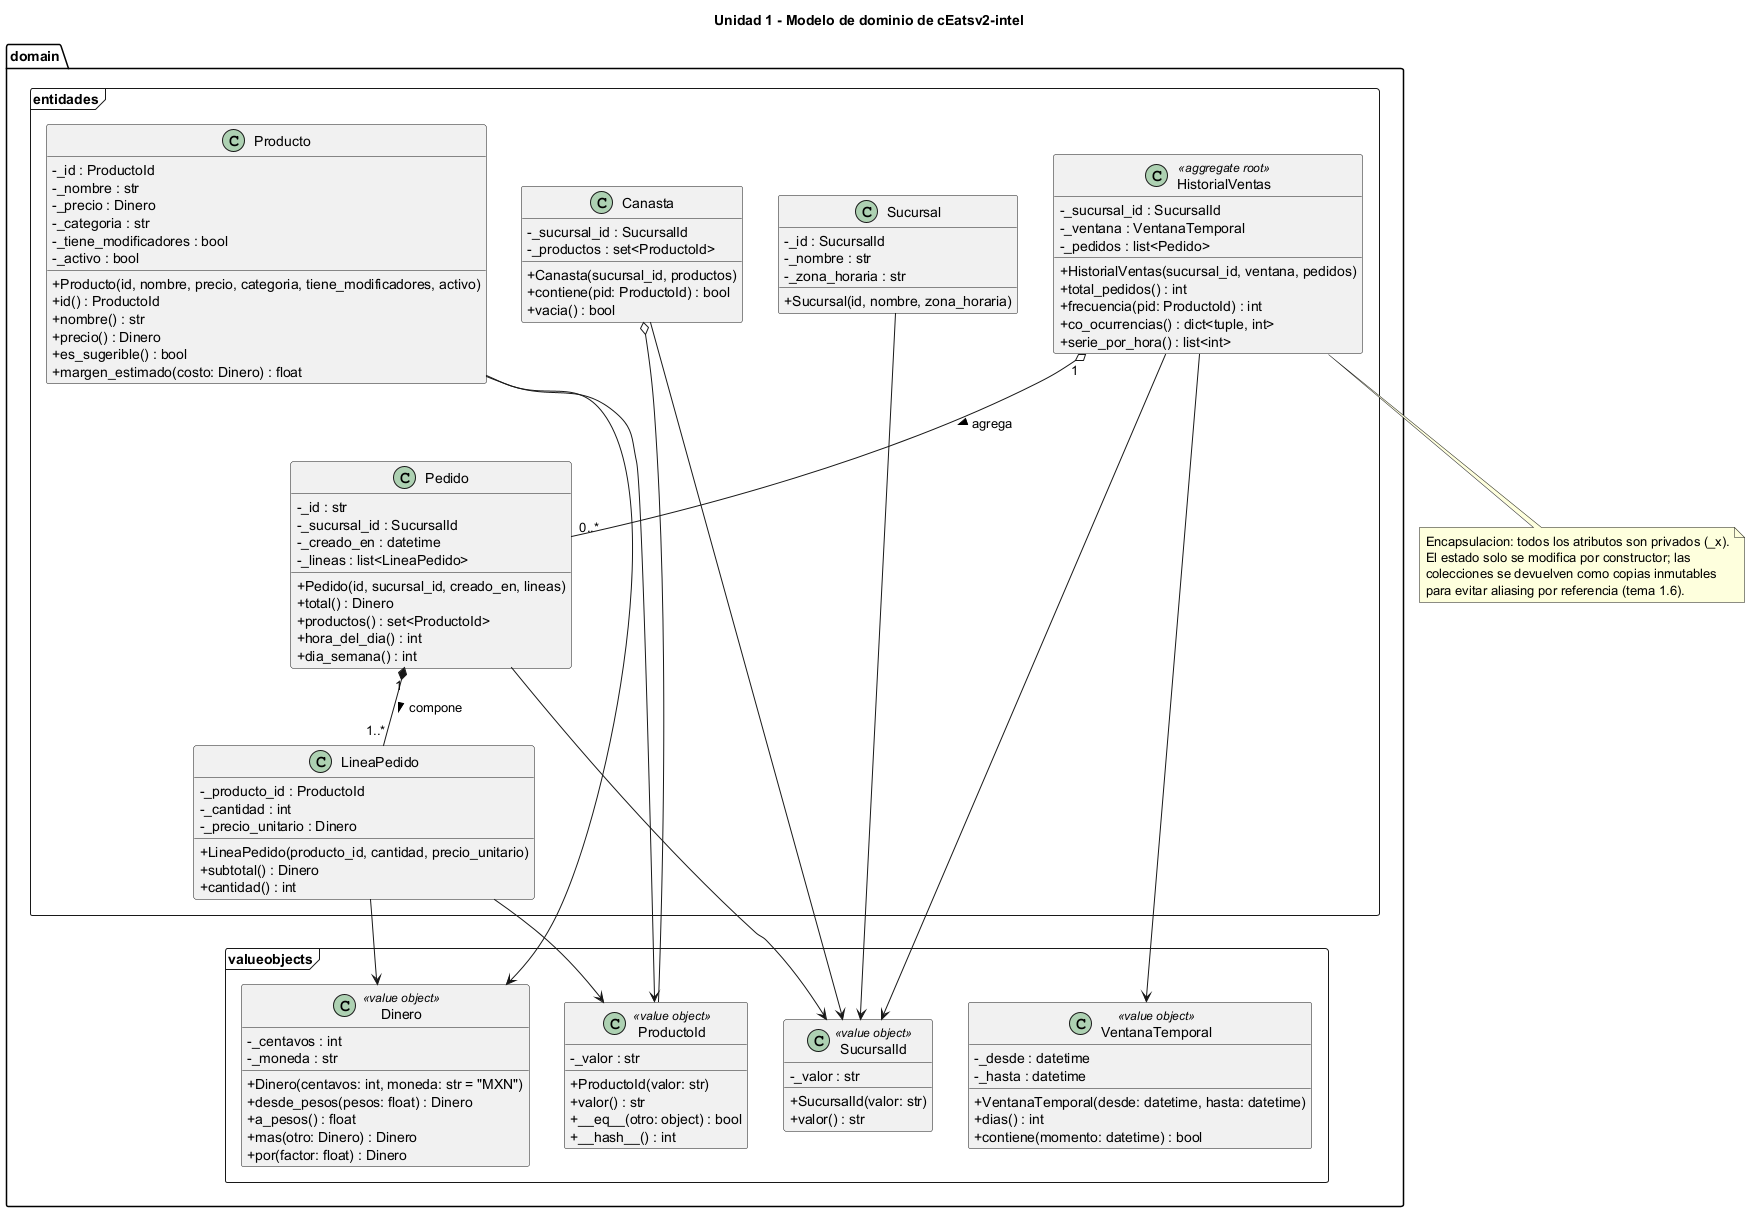
\includegraphics[width=\textwidth]{../uml/png/u1-clases-dominio.png}
\caption{Diagrama de clases del dominio (Unidad 1).}
\label{fig:u1}
\end{figure}

\subsection{Encapsulación y paso por referencia}
Todos los atributos son privados por convención (\texttt{\_atributo}) y se
exponen mediante métodos de acceso. Las colecciones internas nunca se devuelven
por referencia directa: se entregan copias inmutables, para que un consumidor no
pueda mutar el estado del agregado sin pasar por sus métodos. Este es el tema
1.6 del programa: apuntadores, referencias y paso por referencia.

\begin{lstlisting}[caption={Encapsulacion y copia defensiva.}]
class Pedido:
    def __init__(self, id_: str, sucursal_id: SucursalId,
                 creado_en: datetime, lineas: list["LineaPedido"]) -> None:
        if not lineas:
            raise ValueError("Un pedido requiere al menos una linea")
        self._id = id_
        self._sucursal_id = sucursal_id
        self._creado_en = creado_en
        self._lineas = tuple(lineas)   # copia defensiva: evita aliasing

    @property
    def lineas(self) -> tuple["LineaPedido", ...]:
        return self._lineas            # tupla: el consumidor no puede mutar

    def total(self) -> Dinero:
        return reduce(lambda acc, l: acc.mas(l.subtotal()),
                      self._lineas, Dinero.cero())
\end{lstlisting}

\subsection{Modularidad}
La separación en paquetes \texttt{domain}, \texttt{application},
\texttt{infrastructure} y \texttt{api} implementa el principio de inversión de
dependencias: el dominio no importa FastAPI ni \texttt{httpx}, por lo que se
prueba sin levantar un servidor.

\subsection{Evidencia de la unidad}
Rama \texttt{unidad-1}, etiqueta \texttt{v0.1-u1}, diagrama exportado y pruebas
unitarias del dominio.

\newpage
% ------------------------------------------------------------------ UNIDAD 2
\section{Unidad 2 --- Abstracción, herencia y polimorfismo}

\subsection{Resultado de aprendizaje}
Aplicar conceptos de abstracción, herencia y polimorfismo para el diseño de
clases y estructuras complejas.

\begin{figure}[H]
\centering
\includegraphics[width=\textwidth]{../uml/png/u2-herencia-polimorfismo.png}
\caption{Jerarquías polimórficas de recomendación, pronóstico y analítica.}
\label{fig:u2}
\end{figure}

\subsection{Clases abstractas y método plantilla}
\begin{lstlisting}[caption={Clase abstracta con metodo plantilla.}]
class EstrategiaRecomendacion(ABC):
    def __init__(self, nombre: str, peso: float = 1.0) -> None:
        self._nombre = nombre
        self._peso = peso

    @abstractmethod
    def candidatos(self, historial: HistorialVentas,
                   canasta: Canasta) -> list[Candidato]: ...

    @abstractmethod
    def origen(self) -> OrigenSugerencia: ...

    def puntuar(self, historial, canasta, limite: int = 4) -> list[Candidato]:
        """Metodo plantilla comun a todas las subclases."""
        crudos = self.candidatos(historial, canasta)
        pesados = [c.con_score(c.score * self._peso) for c in crudos]
        return heapq.nlargest(limite, pesados, key=lambda c: c.score)
\end{lstlisting}

\subsection{Polimorfismo en el punto de uso}
El caso de uso nunca pregunta por el tipo concreto:

\begin{lstlisting}
estrategia = self._fabrica.crear(peticion.modo)   # tipo abstracto
candidatos = estrategia.puntuar(historial, canasta, peticion.limite)
\end{lstlisting}

\subsection{Sobrecarga}
Python no admite sobrecarga por firma como Java. Se documenta la alternativa
idiomática: \texttt{functools.singledispatchmethod} para despacho por tipo y
parámetros con valor por defecto para variar la aridad.

\subsection{Ciclo de vida de objetos y colecciones}
Las estrategias son efímeras: se construyen por petición y se descartan. El
\texttt{HistorialVentas} se reutiliza desde una caché con tiempo de vida. Se usa
\texttt{dict} para la matriz de co-ocurrencia, \texttt{set} para la canasta y
\texttt{heapq} para el top-N.

\subsection{Evidencia de la unidad}
Rama \texttt{unidad-2}, etiqueta \texttt{v0.2-u2}.

\newpage
% ------------------------------------------------------------------ UNIDAD 3
\section{Unidad 3 --- Cálculo lambda y sus aplicaciones}

\subsection{Resultado de aprendizaje}
Analizar patrones de diseño y fundamentos de la teoría del cálculo lambda.

\begin{figure}[H]
\centering
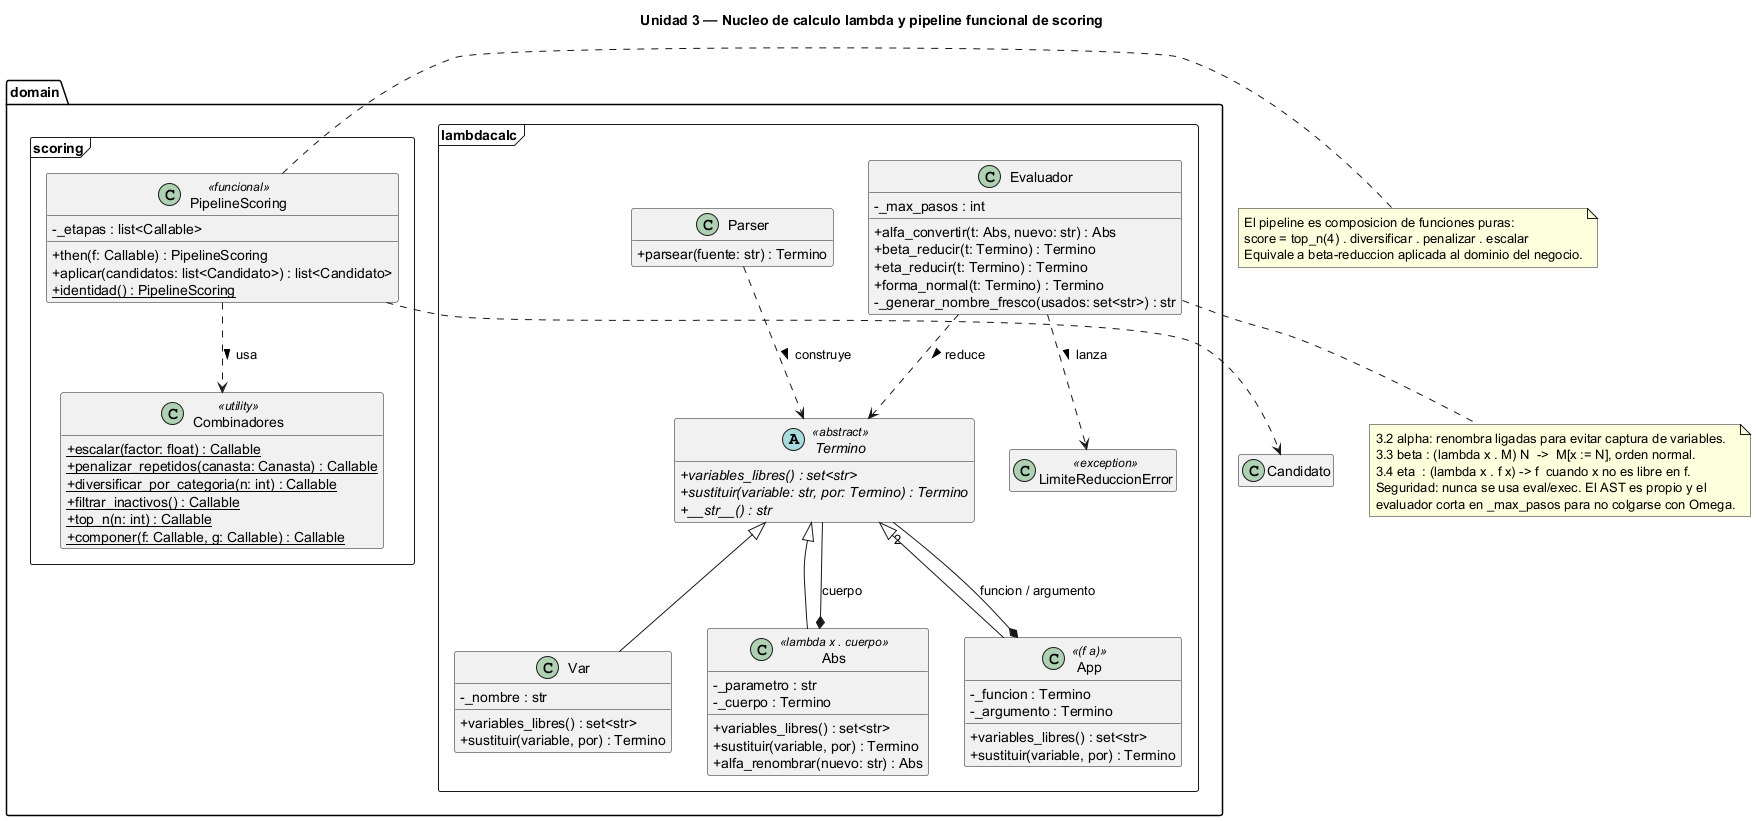
\includegraphics[width=\textwidth]{../uml/png/u3-calculo-lambda.png}
\caption{Núcleo de cálculo lambda y pipeline funcional de scoring.}
\label{fig:u3}
\end{figure}

\subsection{Sintaxis}
Un término $M$ del cálculo lambda se define inductivamente:
\[
M ::= x \;\mid\; (\lambda x.\,M) \;\mid\; (M\;N)
\]
donde $x$ es una variable, $\lambda x.M$ una abstracción y $(M\,N)$ una
aplicación.

\subsection{Conversión alfa}
Renombrado de variables ligadas. Los términos son equivalentes:
\[
\lambda x.\,x \;\equiv_\alpha\; \lambda y.\,y
\]
Se aplica antes de sustituir para evitar la captura de variables.

\subsection{Reducción beta}
\[
(\lambda x.\,M)\,N \;\to_\beta\; M[x := N]
\]

\subsection{Conversión eta}
\[
\lambda x.\,(f\,x) \;\equiv_\eta\; f \qquad \text{si } x \notin FV(f)
\]

\subsection{Aplicación real en el proyecto}
El cálculo del puntaje final se expresa como composición de funciones puras,
que es una reducción beta llevada al dominio del negocio:

\begin{lstlisting}[caption={Pipeline de scoring como composicion de funciones.}]
pipeline = (
    PipelineScoring.identidad()
    .then(Combinadores.filtrar_inactivos())
    .then(Combinadores.penalizar_repetidos(canasta))
    .then(Combinadores.escalar(config.peso_cooccurrencia))
    .then(Combinadores.diversificar_por_categoria(n=2))
    .then(Combinadores.top_n(limite))
)
sugerencias = pipeline.aplicar(candidatos)
\end{lstlisting}

Además se incluye un intérprete propio del cálculo lambda en
\texttt{domain/lambdacalc}, con conversión alfa, reducción beta en orden normal
y conversión eta, verificado por pruebas que reducen los combinadores $I$, $K$ y
$S$ y los numerales de Church.

\subsection{Nota de seguridad}
El intérprete no usa \texttt{eval} ni \texttt{exec}: opera sobre un árbol de
sintaxis propio. El evaluador corta en un número máximo de pasos para no
colgarse ante términos sin forma normal, como
$\Omega = (\lambda x.\,x\,x)(\lambda x.\,x\,x)$.

\subsection{Evidencia de la unidad}
Rama \texttt{unidad-3}, etiqueta \texttt{v0.3-u3}.

\newpage
% ------------------------------------------------------------------ UNIDAD 4
\section{Unidad 4 --- Modelado, patrones y solución aplicada}

\subsection{Resultado de aprendizaje}
Aplicar principios de POO, patrones de diseño y conceptos del cálculo lambda
para resolver un problema aplicado en ciencia de datos.

\begin{figure}[H]
\centering
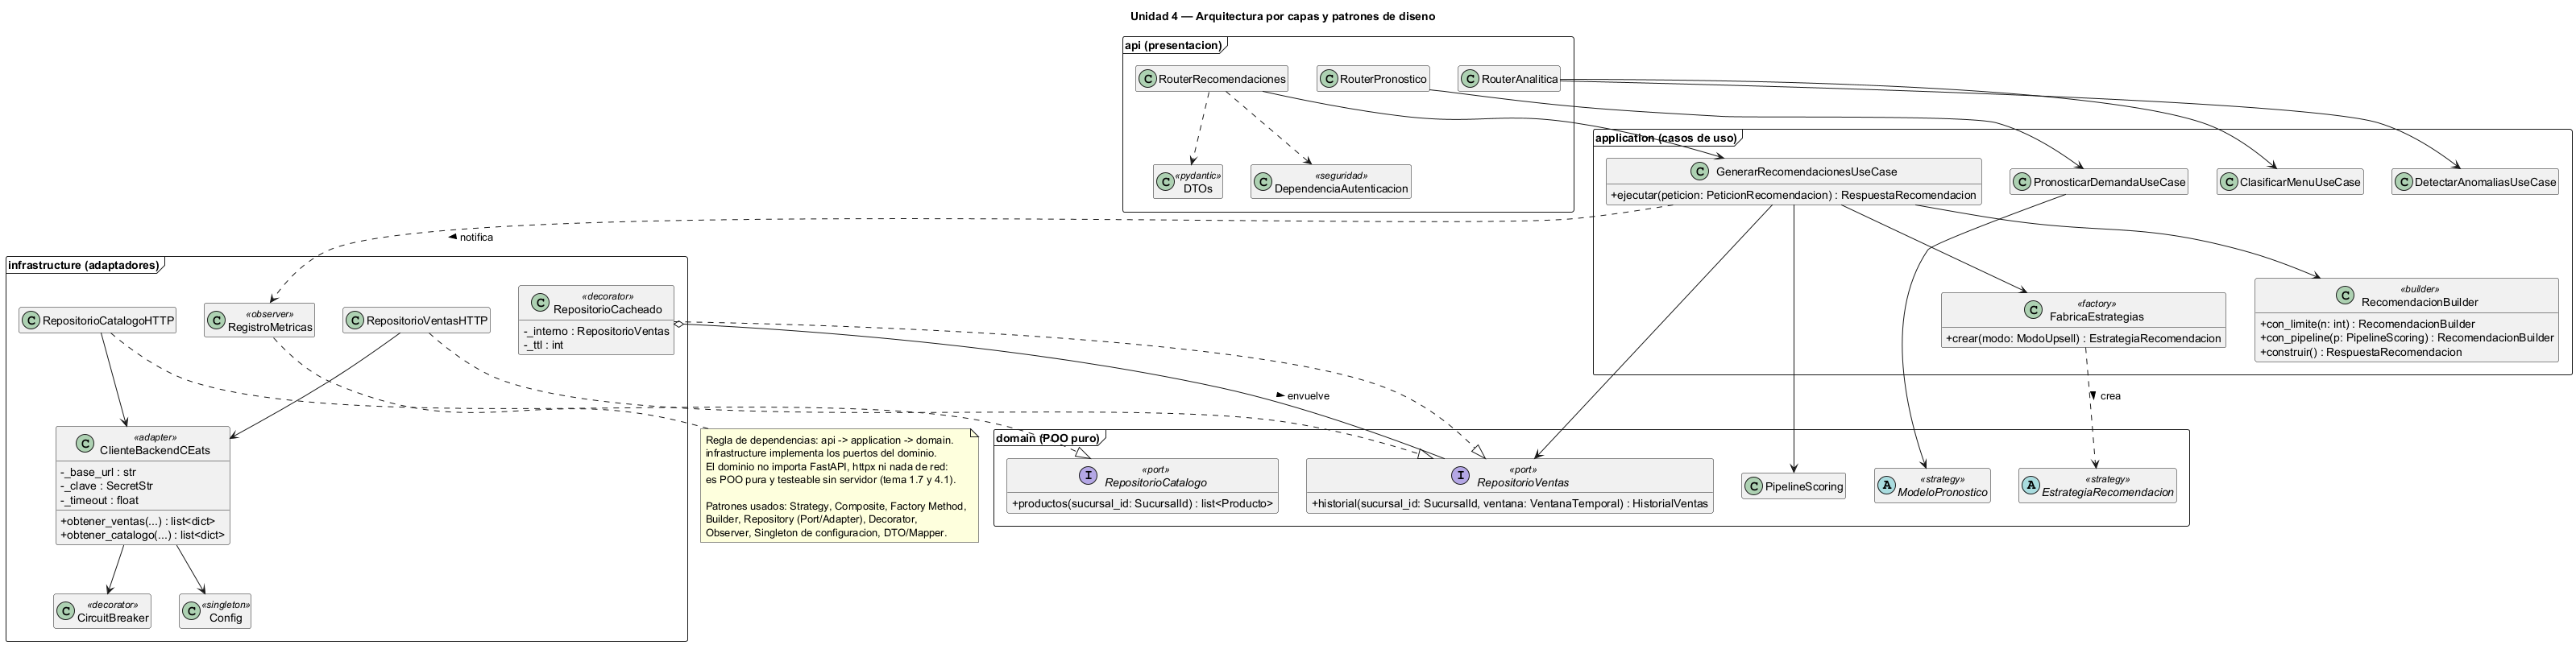
\includegraphics[width=\textwidth]{../uml/png/u4-patrones-y-capas.png}
\caption{Arquitectura por capas y patrones de diseño.}
\label{fig:u4}
\end{figure}

\subsection{Patrones aplicados}
\begin{longtable}{@{}p{3.4cm}p{5.2cm}p{5.6cm}@{}}
\toprule
\textbf{Patrón} & \textbf{Dónde} & \textbf{Por qué} \\
\midrule
\endhead
Strategy & \texttt{EstrategiaRecomendacion}, \texttt{ModeloPronostico} & Intercambiar el algoritmo sin tocar el caso de uso. \\
Composite & \texttt{HibridaStrategy} & Combinar reglas manuales y automáticas con la misma interfaz. \\
Factory Method & \texttt{FabricaEstrategias} & Resolver el modo configurado a una instancia concreta. \\
Builder & \texttt{RecomendacionBuilder} & Armar la respuesta paso a paso. \\
Repository & \texttt{RepositorioVentas} & Aislar el dominio del origen de datos. \\
Decorator & \texttt{RepositorioCacheado}, \texttt{CircuitBreaker} & Añadir caché y tolerancia a fallos sin modificar el adaptador. \\
Observer & \texttt{RegistroMetricas} & Publicar métricas sin acoplar el caso de uso. \\
Adapter & \texttt{ClienteBackendCEats} & Traducir el contrato HTTP del backend al dominio. \\
\bottomrule
\end{longtable}

\subsection{Ciencia de datos aplicada}
\paragraph{Análisis de canasta de mercado.} Para dos productos $A$ y $B$ sobre
$N$ pedidos:
\[
\mathrm{sop}(A \to B)=\frac{n(A \cap B)}{N}, \quad
\mathrm{conf}(A \to B)=\frac{n(A \cap B)}{n(A)}, \quad
\mathrm{lift}(A \to B)=\frac{\mathrm{conf}(A \to B)}{\mathrm{sop}(B)}
\]
Se sugiere $B$ sólo si $\mathrm{lift} > 1$ y el soporte supera un mínimo.

\paragraph{Pronóstico de demanda.} Media móvil, perfil estacional semanal y
regresión lineal, evaluados con el error absoluto medio:
\[
\mathrm{MAE} = \frac{1}{n}\sum_{i=1}^{n}\left| y_i - \hat{y}_i \right|
\]

\paragraph{Detección de anomalías.} Puntaje $z$ sobre la serie de ventas:
\[
z_i = \frac{x_i - \mu}{\sigma}, \qquad \text{se alerta si } |z_i| > 3
\]

\subsection{Desarrollo colaborativo}
Repositorio Git independiente, una rama por unidad, \emph{pull requests}
revisados, etiquetas de entrega y bitácora de cambios.

\subsection{Despliegue}
\begin{figure}[H]
\centering
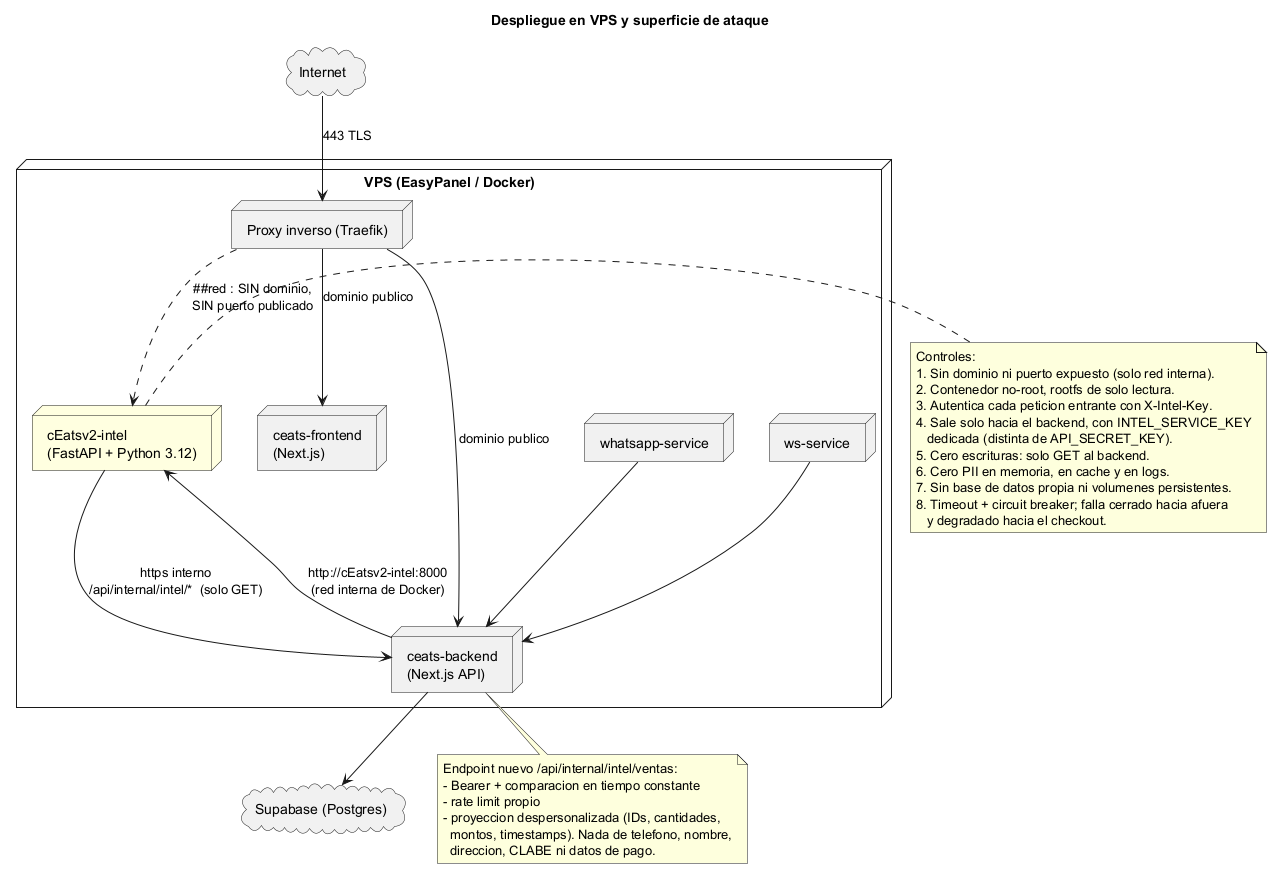
\includegraphics[width=\textwidth]{../uml/png/despliegue-y-seguridad.png}
\caption{Despliegue en el VPS y superficie de ataque.}
\label{fig:deploy}
\end{figure}

\begin{figure}[H]
\centering
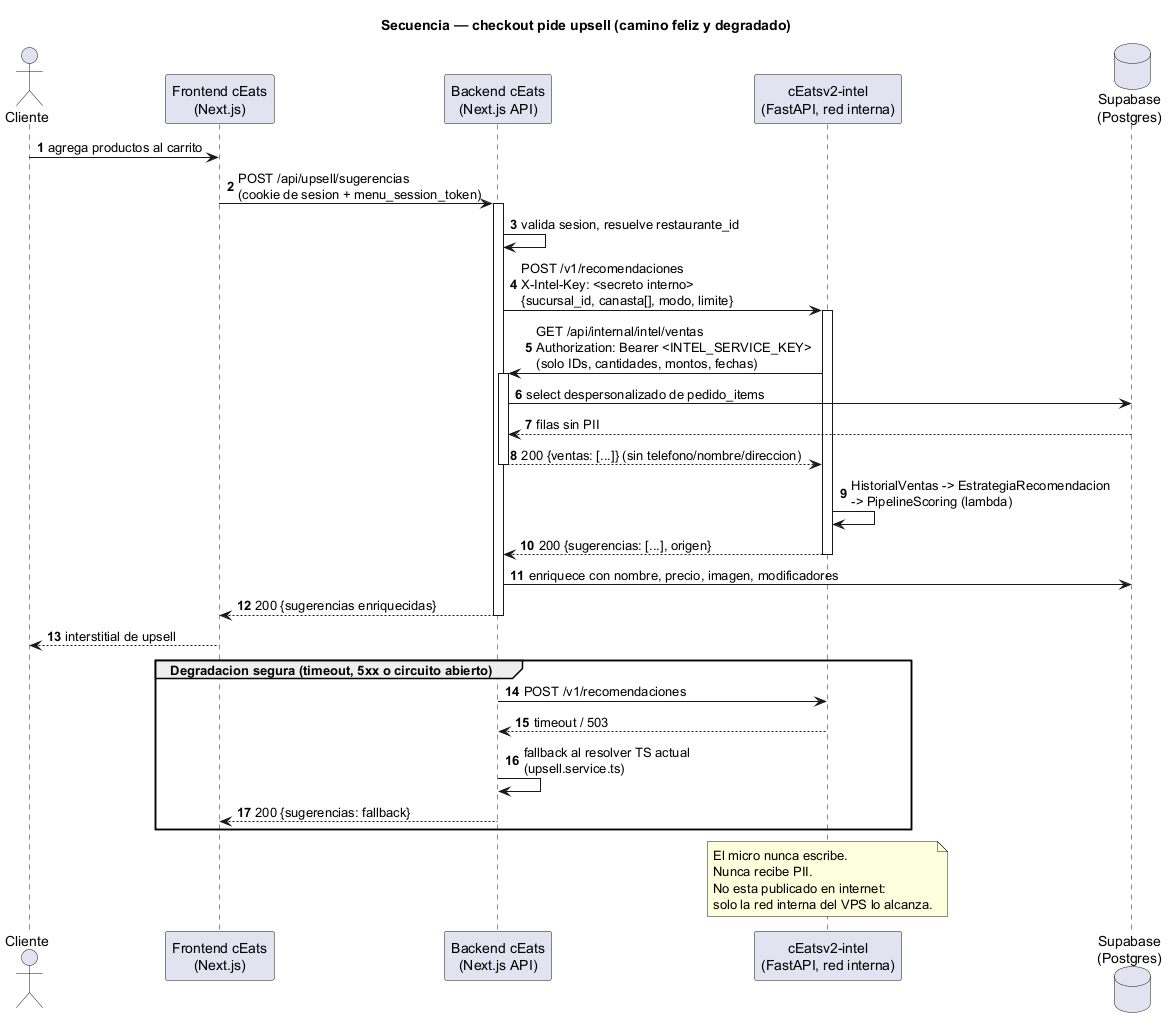
\includegraphics[width=\textwidth]{../uml/png/secuencia-recomendacion.png}
\caption{Secuencia de una petición de upsell con degradación segura.}
\label{fig:seq}
\end{figure}

\section{Seguridad}
El modelo de amenazas completo está en \texttt{SEGURIDAD.md}, en la raíz del
repositorio. En resumen: el microservicio no se publica a internet, no escribe
nada, no recibe datos personales, autentica toda petición entrante y usa un
secreto dedicado --- distinto del secreto general del backend --- para sus
lecturas.

\section{Conclusiones}

\begin{thebibliography}{9}
\bibitem{rojas} Rojas, R. (2015). \emph{A tutorial introduction to the lambda calculus}. arXiv:1503.09060.
\bibitem{gof} Gamma, E., Helm, R., Johnson, R., \& Vlissides, J. (1994). \emph{Design patterns}. Addison-Wesley.
\bibitem{weisfeld} Weisfeld, M. (2019). \emph{The object-oriented thought process} (5th ed.). Addison-Wesley.
\bibitem{pressman} Pressman, R. S., \& Maxim, B. R. (2020). \emph{Ingeniería del software: un enfoque práctico} (9.ª ed.). McGraw-Hill.
\bibitem{sicp} Abelson, H., \& Sussman, G. J. (2022). \emph{Structure and interpretation of computer programs: JavaScript edition}. MIT Press.
\end{thebibliography}

\end{document}
